\subsection{Análise Descritiva e dos Fatores Experimentais}

A inspeção inicial dos dados revela padrões distribucionais que justificam a adoção de métodos não-paramétricos robustos. A Figura \ref{fig:distribuicao_metricas} apresenta os histogramas de frequência para as cinco métricas de avaliação.

\begin{figure}[h]
  \centering
  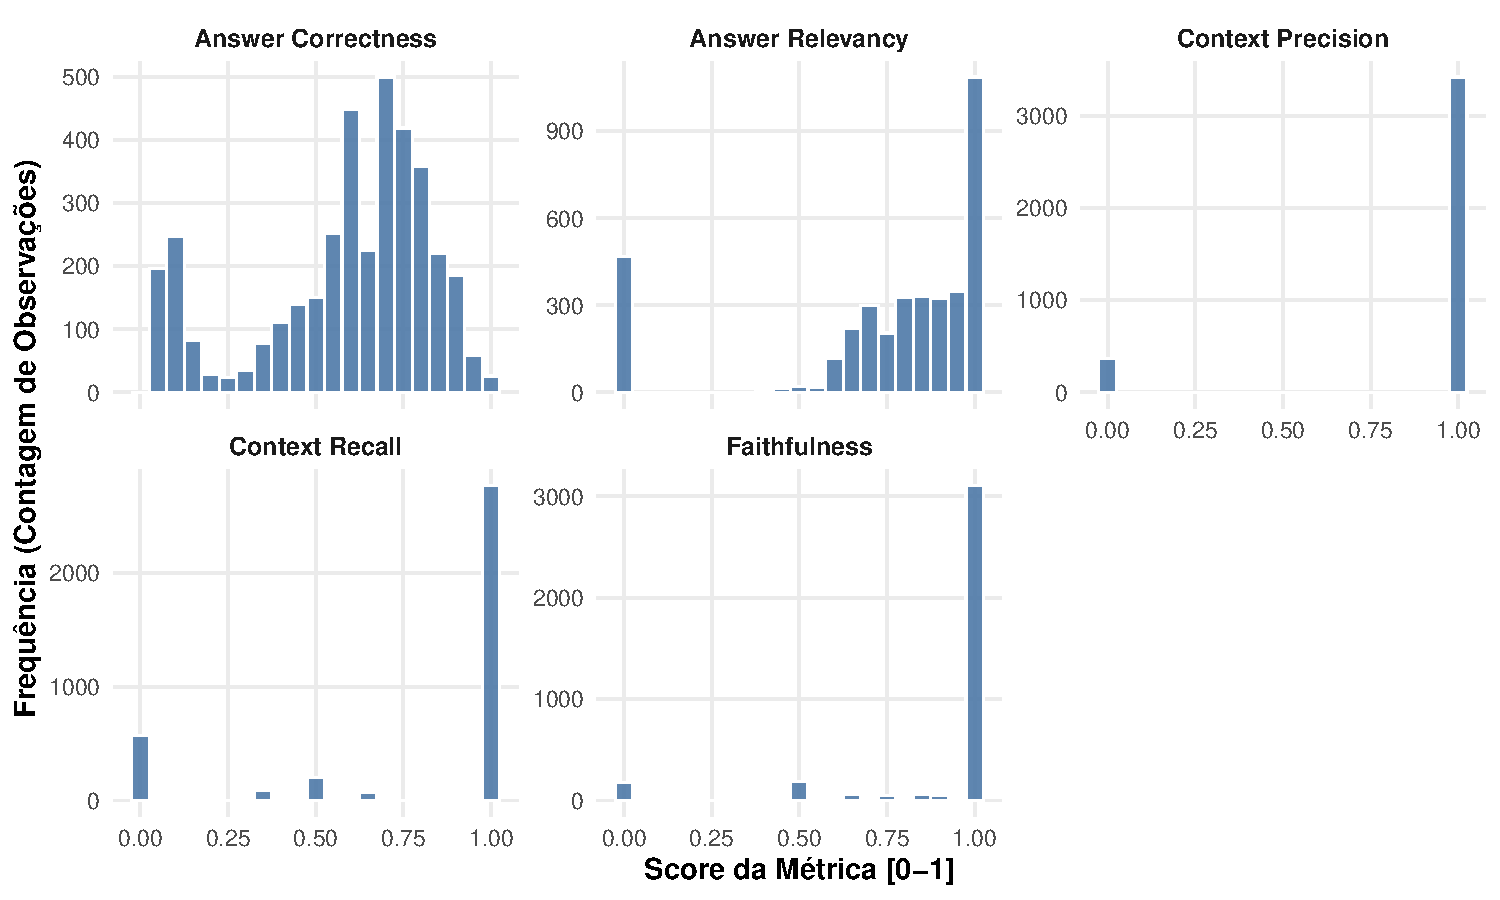
\includegraphics[width=0.8\textwidth]{figuras/distribuicao_metricas.pdf}
  \caption{Distribuição de Frequência das Métricas de Avaliação.}
  \label{fig:distribuicao_metricas}
  \small \textbf{Fonte:} Elaborado pelo autor.
\end{figure}

A análise visual permite três diagnósticos fundamentais: (i) as métricas de recuperação exibem um comportamento polarizado (``tudo ou nada''), com concentração massiva em 1,0; (ii) a \textit{Faithfulness} demonstra que os modelos testados raramente alucinam, mantendo alta aderência factual; e (iii) a \textit{Answer Correctness} apresenta multimodalidade, refletindo sua natureza híbrida que penaliza erros factuais mesmo em respostas coerentes.

A seguir, detalha-se o impacto isolado de cada hiperparâmetro, com as médias organizadas pelas etapas do \textit{pipeline} RAG: Recuperação, Geração e Avaliação Global.

\subsubsection{Estratégia de Segmentação (\textit{Chunking})}

A Tabela \ref{tab:chunking_results} apresenta os resultados por estratégia de particionamento. Observa-se que a fragmentação excessiva (\textit{Recursive 500}) gera o pior desempenho em todas as dimensões. Em contrapartida, a abordagem \textit{Semantic (P95)} obteve o maior \textit{Recall} médio (0,89), sugerindo que janelas baseadas em mudanças de tópico preservam melhor a completude da informação jurídica.

\begin{table}[h]
  \centering
  \caption{Desempenho médio por Estratégia de \textit{Chunking}.}
  \label{tab:chunking_results}
  \small
  \begin{tabular}{lccccc}
    \toprule
    & \multicolumn{2}{c}{\textbf{Recuperação}} & \multicolumn{2}{c}{\textbf{Geração}} & \textbf{Global} \\ \cmidrule(lr){2-3} \cmidrule(lr){4-5} \cmidrule(l){6-6}
    \textbf{Estratégia} & \textbf{Recall} & \textbf{Precision} & \textbf{Faithful.} & \textbf{Relevancy} & \textbf{Correct.} \\ \midrule
    Recursive (1000) & 0,81 & \textbf{0,94} & \textbf{0,95} & \textbf{0,78} & 0,61 \\
    Recursive (500)  & 0,65 & 0,86 & 0,89 & 0,71 & 0,52 \\
    Semantic (P75)   & 0,81 & 0,87 & 0,88 & 0,74 & 0,59 \\
    Semantic (P95)   & \textbf{0,89} & 0,93 & 0,91 & 0,77 & \textbf{0,62} \\ \bottomrule
  \end{tabular}
\end{table}

\subsubsection{Estratégia de Busca}

A Tabela \ref{tab:search_results} apresenta o desempenho comparativo entre os algoritmos de busca. A \textbf{Busca Híbrida} superou as abordagens isoladas em todas as categorias, demonstrando que a combinação da precisão terminológica do BM25 com a abrangência semântica dos vetores resulta em um sistema mais robusto para o domínio jurídico.

\begin{table}[ht]
  \centering
  \caption{Desempenho médio por Tipo de Busca.}
  \label{tab:search_results}
  \small
  \begin{tabular}{lccccc}
    \toprule
    & \multicolumn{2}{c}{\textbf{Recuperação}} & \multicolumn{2}{c}{\textbf{Geração}} & \textbf{Global} \\ \cmidrule(lr){2-3} \cmidrule(lr){4-5} \cmidrule(l){6-6}
    \textbf{Algoritmo} & \textbf{Recall} & \textbf{Precision} & \textbf{Faithful.} & \textbf{Relevancy} & \textbf{Correct.} \\ \midrule
    Híbrida  & \textbf{0,83} & \textbf{0,93} & \textbf{0,93} & \textbf{0,78} & \textbf{0,62} \\
    Textual  & 0,74 & 0,86 & 0,89 & 0,73 & 0,55 \\
    Vetorial & 0,80 & 0,92 & 0,91 & 0,75 & 0,60 \\ \bottomrule
  \end{tabular}
\end{table}

\subsubsection{Janela de Contexto (Top-K)}

O impacto do volume de contexto recuperado é detalhado na Tabela \ref{tab:topk_results}. Observa-se um crescimento consistente e linear dos escores conforme a janela se expande. O limite de \textbf{Top-20} apresentou os melhores resultados, indicando que, para o conjunto de dados do MPES, o benefício da informação adicional supera o risco de introdução de ruído no \textit{prompt}.

\begin{table}[ht]
  \centering
  \caption{Desempenho médio por Tamanho da Janela (Top-K).}
  \label{tab:topk_results}
  \small
  \begin{tabular}{lccccc}
    \toprule
    & \multicolumn{2}{c}{\textbf{Recuperação}} & \multicolumn{2}{c}{\textbf{Geração}} & \textbf{Global} \\ \cmidrule(lr){2-3} \cmidrule(lr){4-5} \cmidrule(l){6-6}
    \textbf{Nível} & \textbf{Recall} & \textbf{Precision} & \textbf{Faithful.} & \textbf{Relevancy} & \textbf{Correct.} \\ \midrule
    Top-5  & 0,70 & 0,83 & 0,88 & 0,71 & 0,54 \\
    Top-10 & 0,79 & 0,91 & \textbf{0,92} & 0,76 & 0,59 \\
    Top-15 & 0,82 & 0,93 & 0,91 & 0,77 & 0,60 \\
    Top-20 & \textbf{0,85} & \textbf{0,94} & \textbf{0,92} & \textbf{0,78} & \textbf{0,62} \\ \bottomrule
  \end{tabular}
\end{table}
\subsubsection{Modelo LLM}

A Tabela \ref{tab:model_results} valida a eficiência do modelo \textbf{GPT-4o-mini}, que apresentou desempenho superior em métricas de geração e corretude global, consolidando-se como a melhor opção de custo-benefício para o domínio jurídico do MPES.

\begin{table}[h]
  \centering
  \caption{Desempenho médio por Modelo LLM.}
  \label{tab:model_results}
  \small
  \begin{tabular}{lccccc}
    \toprule
    & \multicolumn{2}{c}{\textbf{Recuperação}} & \multicolumn{2}{c}{\textbf{Geração}} & \textbf{Global} \\ \cmidrule(lr){2-3} \cmidrule(lr){4-5} \cmidrule(l){6-6}
    \textbf{Modelo} & \textbf{Recall} & \textbf{Precision} & \textbf{Faithful.} & \textbf{Relevancy} & \textbf{Correct.} \\ \midrule
    GPT-4o      & 0,79 & 0,90 & 0,90 & 0,73 & 0,58 \\
    GPT-4o-mini & 0,79 & 0,90 & \textbf{0,92} & \textbf{0,78} & \textbf{0,60} \\ \bottomrule
  \end{tabular}
\end{table}
